\documentclass[conference]{IEEEtran}
\IEEEoverridecommandlockouts
\usepackage{cite}
\usepackage{amsmath,amssymb,amsfonts}
\usepackage{graphicx}
\usepackage{textcomp}
\usepackage{xcolor}
\usepackage{booktabs}
\usepackage{multirow}
\usepackage{url}
\usepackage[hidelinks]{hyperref}

% Line break between author rows (not defined in older IEEEtran releases)
\makeatletter
\providecommand{\linebreakand}{%
  \end{@IEEEauthorhalign}
  \hfill\mbox{}\par
  \mbox{}\hfill\begin{@IEEEauthorhalign}
}
\makeatother

\begin{document}

\title{Supervised Machine Learning for Multi-Component Condition Classification in Industrial Hydraulic Systems}

\author{
\IEEEauthorblockN{Sahil Khan Pathan}
\IEEEauthorblockA{\textit{Roll No. 24AD1199}}
\and
\IEEEauthorblockN{Vedant Mali}
\IEEEauthorblockA{\textit{Roll No. 24AD1145}}
\and
\IEEEauthorblockN{Sejal Zende}
\IEEEauthorblockA{\textit{Roll No. 24AD1158}}
\and
\IEEEauthorblockN{Vedika Singh}
\IEEEauthorblockA{\textit{Roll No. 24AD1147}}
\linebreakand
\IEEEauthorblockA{\textit{Department of Artificial Intelligence and Data Science Engineering}\\
\textit{DY Patil University}, Navi Mumbai, India}
}

\maketitle

\begin{abstract}
Unplanned failures of hydraulic power units stop the production lines they
drive, which makes data-driven condition monitoring an attractive alternative
to fixed-interval maintenance. This paper frames the condition monitoring of a
hydraulic test rig as four independent supervised multiclass classification
problems---cooler efficiency, valve switching behaviour, internal pump leakage
and accumulator gas pre-charge pressure---and studies how four classifier
families behave on them: multinomial logistic regression, random forest,
gradient-boosted trees (XGBoost) and an RBF-kernel support vector machine. Each
60-second operating cycle of 17 sensors (43{,}680 raw values) is mapped to a
fixed-length input vector, and every learned transformation, including feature
selection, is fitted inside a single pipeline to prevent train--validation
leakage. Using 2{,}205 cycles, model selection by stratified 5-fold
cross-validation on an 80\,\% training split yields macro-F1 scores between
0.992 and 0.998, and the selected models reach a held-out macro-F1 of 1.000
for the cooler, valve and pump and 0.988 for the accumulator. A blocked
cross-validation that holds out contiguous runs of cycles lowers these
estimates to 0.995, 0.984, 0.968 and 0.916 respectively, exposing an
optimism of up to 7.6 points in randomly split evaluation. The results show
that the accumulator is the hardest target, that linear and kernel models
are the most sensitive to the input representation, and that temporally
aware validation should be reported alongside random-split scores.
\end{abstract}

\begin{IEEEkeywords}
predictive maintenance, condition monitoring, hydraulic systems, multiclass
classification, random forest, gradient boosting, support vector machine,
cross-validation, data leakage
\end{IEEEkeywords}

%=====================================================================
\section{Introduction}
%=====================================================================
Hydraulic power units supply force and motion to presses, injection-moulding
machines and mobile equipment. Their components degrade gradually: coolers
foul, valves develop switching lag, pumps leak internally and accumulators
lose gas pre-charge. Because degradation leaves a signature in routinely
measured pressures, flows, temperatures and motor power, it can in principle be
recognised by a statistical model long before a functional failure occurs.
Machine learning (ML) is now the dominant tool for this kind of predictive
maintenance \cite{carvalho2019}.

The public dataset released by Helwig \textit{et al.}
\cite{helwig2015,uci_hydraulic} records such a rig under systematically varied
component conditions, and has become a standard benchmark. Two properties make
it demanding from an ML perspective. First, each observation is a multi-rate
multivariate time series with far more raw values (43{,}680) than there are
observations (2{,}205), so a classifier cannot consume it directly. Second,
consecutive cycles are recorded seconds apart under identical settings, so
observations are not independent and randomly split evaluation can be
optimistic \cite{kaufman2012,roberts2017}.

This work treats the problem primarily as a supervised learning and model
evaluation study. Its contributions are:
\begin{itemize}
\item a leakage-safe learning pipeline in which imputation, scaling,
three-stage feature selection and the classifier are fitted jointly, so
cross-validation estimates the whole procedure rather than the classifier
alone;
\item a controlled comparison of four classifier families on three input
representations for each of four targets (48 configurations), with
hyperparameters held fixed so that differences are attributable to model
family and representation;
\item a blocked cross-validation analysis that quantifies how much randomly
split scores overstate generalisation on this dataset; and
\item an error and interpretability analysis of the selected models, deployed
behind an inference-only dashboard.
\end{itemize}

%=====================================================================
\section{Related Work}
%=====================================================================
Helwig \textit{et al.} \cite{helwig2015} introduced the rig and classified its
component states with linear discriminant analysis on statistical and
spectral features, reporting high accuracy for most fault types and lower
accuracy for the accumulator. Their work established that hand-crafted cycle
statistics carry most of the discriminative information. Subsequent studies on
the same data have applied ensemble learners and deep networks, but frequently
report only randomly split accuracy.

Among general-purpose tabular learners, random forests \cite{breiman2001} and
gradient-boosted trees such as XGBoost \cite{chen2016} are strong defaults
because they model feature interactions and are insensitive to monotone
transformations of the inputs. Support vector machines \cite{cortes1995}
remain competitive on small, well-scaled datasets. Carvalho \textit{et al.}
\cite{carvalho2019} survey their use in predictive maintenance and note that
random forest is the most frequently applied method in that literature.

Leakage---information about the evaluation data reaching the training
procedure---is a recognised source of inflated results \cite{kaufman2012}.
For data with temporal or grouped structure, Roberts \textit{et al.}
\cite{roberts2017} recommend blocked cross-validation, in which whole blocks of
dependent observations are held out together. We apply that recommendation as
a diagnostic.

%=====================================================================
\section{Dataset and Problem Formulation}
%=====================================================================
\subsection{Data}
The rig repeats a constant 60-s load cycle while 17 channels are logged
(Table~\ref{tab:sensors}): six pressure sensors and motor power at 100~Hz, two
flow sensors at 10~Hz, and four temperatures, a vibration channel and three
rig-computed virtual quantities at 1~Hz. One cycle therefore holds
$7\times6000 + 2\times600 + 8\times60 = 43{,}680$ values. The dataset contains
$N = 2{,}205$ cycles with no missing values.

\begin{table}[t]
\centering
\caption{Sensor channels per operating cycle}
\label{tab:sensors}
\begin{tabular}{@{}llcc@{}}
\toprule
Channels & Quantity & Rate [Hz] & Samples \\
\midrule
PS1--PS6 & Pressure [bar] & 100 & 6000 \\
EPS1 & Motor power [W] & 100 & 6000 \\
FS1, FS2 & Volume flow [l/min] & 10 & 600 \\
TS1--TS4 & Temperature [\textdegree C] & 1 & 60 \\
VS1 & Vibration [mm/s] & 1 & 60 \\
CE, CP, SE & Virtual (efficiency, power) & 1 & 60 \\
\bottomrule
\end{tabular}
\end{table}

\subsection{Targets}
Each cycle carries four condition labels (Table~\ref{tab:targets}). They are
modelled as four independent multiclass problems rather than one joint label,
because the joint label space has $3\times4\times3\times4=144$ combinations,
most of which occur in only 10 cycles (median 10, maximum 230), and because
each component is serviced separately. For a target
$k$ with class set $\mathcal{C}_k$, we learn
$f_k:\mathbb{R}^{d}\rightarrow\mathcal{C}_k$ from pairs
$(\mathbf{x}_i, y_i^{(k)})$, $i=1,\dots,N$.

\begin{table}[t]
\centering
\caption{Prediction targets and class balance}
\label{tab:targets}
\begin{tabular}{@{}lccc@{}}
\toprule
Target & Classes & Class counts & $\rho$ \\
\midrule
Cooler [\%] & 3 / 20 / 100 & 732 / 732 / 741 & 1.01 \\
Valve [\%] & 73 / 80 / 90 / 100 & 360 / 360 / 360 / 1125 & 3.13 \\
Pump leakage & 0 / 1 / 2 & 1221 / 492 / 492 & 2.48 \\
Accumulator [bar] & 90 / 100 / 115 / 130 & 808 / 399 / 399 / 599 & 2.03 \\
\bottomrule
\multicolumn{4}{@{}l}{\footnotesize $\rho$: imbalance ratio, largest / smallest class.}
\end{tabular}
\end{table}

A separate stable-flag marks 756 cycles in which static conditions may not
have been reached. It describes the rig rather than a component and is kept as
metadata. The dataset annotates condition levels, not failure times, so
remaining useful life cannot be estimated and is out of scope.

%=====================================================================
\section{Methodology}
%=====================================================================
\subsection{Input Representation}
Because the channels are sampled at different rates, raw sample positions are
not aligned in time and cannot serve directly as features. Each cycle is
summarised by a fixed-length vector of 626 descriptors in five groups:
distribution statistics (mean, quantiles, RMS, skewness, kurtosis),
time-domain descriptors (slope, first-difference statistics, peak counts),
1-s rolling-window statistics, a compact FFT summary (dominant frequency,
spectral centroid, log-spaced band-energy ratios) and physically motivated
cross-channel quantities (pressure differentials, flow imbalance, hydraulic
power and electro-hydraulic efficiency). Unsupervised cleaning removes 4
constant, 4 near-constant and 65 exactly duplicated columns, leaving
$d=553$. Three representations are compared:
\begin{itemize}
\item \textit{Baseline}: the 17 per-channel cycle means ($d=17$);
\item \textit{Full}: all 553 cleaned descriptors;
\item \textit{Selected}: the 553 descriptors passed through the in-pipeline
selector of Section~\ref{sec:selection}, which outputs 40.
\end{itemize}

\subsection{Leakage-Safe Pipeline}
Every learned step is a stage of one scikit-learn \texttt{Pipeline}
\cite{pedregosa2011}: median imputation, standardisation
$z_j=(x_j-\mu_j)/\sigma_j$, the optional selector and the classifier. Calling
\texttt{fit} on a training fold therefore re-estimates imputation medians,
scaling moments, selection masks and model parameters from that fold only, and
cross-validation scores the complete procedure. The only steps fitted on all
cycles are the label-free column removals above, which cannot use target
information.

\subsection{Feature Selection as Part of the Model}
\label{sec:selection}
The \textit{Selected} representation applies three filters in sequence, each
fitted on training data:
\begin{enumerate}
\item \textit{Correlation filter}: scanning columns in order, a column is
dropped if $|r|>0.95$ with any column already kept, which removes
near-duplicates (553$\,\rightarrow\,$about 237).
\item \textit{Mutual information}: the top 50\,\% of columns by estimated
$I(X_j;Y)$ are retained \cite{kraskov2004}, a model-free relevance ranking that
captures non-linear dependence (about 118 columns).
\item \textit{Embedded tree importance}: a 200-tree random forest ranks the
survivors by mean impurity decrease and the top $k=40$ are passed on. Unlike
the univariate filter, this scores each feature in the context of the others.
\end{enumerate}

\subsection{Classifiers}
Four model families with different inductive biases are compared.
Hyperparameters are fixed (Table~\ref{tab:hyper}) rather than tuned per target,
so that the 48 configurations differ only in model family and representation.

\textit{Multinomial logistic regression} (LR) models
$P(y=c\mid\mathbf{x})=\exp(\mathbf{w}_c^{\top}\mathbf{x}+b_c)/
\sum_{c'}\exp(\mathbf{w}_{c'}^{\top}\mathbf{x}+b_{c'})$ with $\ell_2$
regularisation. As a linear model it cannot construct interactions, so its
score is a direct probe of how linearly separable a representation is.

\textit{Random forest} (RF) \cite{breiman2001} averages $B=300$ decorrelated
decision trees grown on bootstrap samples with random feature subsets.

\textit{Gradient boosting} (XGB) \cite{chen2016} builds an additive model
$F_M(\mathbf{x})=\sum_{m=1}^{M}\eta\,h_m(\mathbf{x})$ by fitting each tree
$h_m$ to the gradient of the regularised multiclass log-loss
\begin{equation}
\mathcal{L}=\sum_{i} \ell\bigl(y_i,F(\mathbf{x}_i)\bigr)+\sum_{m}\Omega(h_m),\quad
\Omega(h)=\gamma T+\tfrac{1}{2}\lambda\lVert\mathbf{w}\rVert^2,
\end{equation}
where $\Omega$ penalises the number of leaves $T$ and the leaf weights
$\mathbf{w}$.

\textit{Support vector machine} (SVM) \cite{cortes1995} uses the RBF kernel
$K(\mathbf{x},\mathbf{x}')=\exp(-\gamma\lVert\mathbf{x}-\mathbf{x}'\rVert^2)$
with one-vs-one decomposition for multiple classes.

\begin{table}[t]
\centering
\caption{Fixed classifier hyperparameters}
\label{tab:hyper}
\begin{tabular}{@{}ll@{}}
\toprule
Model & Settings \\
\midrule
LR & $\ell_2$, $C=1$, L-BFGS, 3000 iterations \\
RF & 300 trees, unlimited depth, min.\ leaf size 1 \\
XGB & 300 trees, depth 5, $\eta=0.1$, subsample 0.9, \\
    & column sample 0.8, histogram tree method \\
SVM & RBF, $C=10$, $\gamma=1/(d\,\mathrm{Var}[X])$ \\
\bottomrule
\end{tabular}
\end{table}

\subsection{Class Imbalance}
When the imbalance ratio $\rho$ exceeds 1.5 (valve, pump, accumulator), each
class $c$ receives weight $w_c=N/(|\mathcal{C}|\,N_c)$. LR, RF and SVM use
this through their \texttt{class\_weight} option. Because XGBoost accepts only
per-sample weights, a thin wrapper computes $w_{y_i}$ inside \texttt{fit} from
the labels of the current fold, so weights never depend on validation data.
The near-uniform cooler target is left unweighted.

\subsection{Evaluation Protocol and Metrics}
For each target, the cycles are split once into 80\,\% training (1{,}764) and
20\,\% test (441), stratified by class. Model selection uses stratified 5-fold
cross-validation on the training set only; the configuration with the highest
mean CV macro-F1 is selected (ties go to the simpler representation and
model), refitted on the full training set, and scored exactly once on the
test set.

The headline metric is the macro-averaged F1 score,
\begin{equation}
\mathrm{F1}_{\text{macro}}=\frac{1}{|\mathcal{C}|}\sum_{c\in\mathcal{C}}
\frac{2\,P_c R_c}{P_c+R_c},
\end{equation}
where $P_c$ and $R_c$ are the precision and recall of class $c$. It weights
every condition level equally, which matters because the rare severe-fault
classes are the costly ones. Accuracy, weighted F1 and one-vs-rest ROC-AUC are
also reported.

\subsection{Blocked Cross-Validation}
Neighbouring cycles share operating settings and slowly drifting temperatures,
so a random fold assignment places near-identical cycles on both sides of the
split. To measure the effect, the cycle index is partitioned into contiguous
blocks of 25 cycles and \texttt{StratifiedGroupKFold} (5 folds) is run with the
block as the group over all 2{,}205 cycles, so a validation cycle's immediate
neighbours are never in the training folds except at block boundaries. This
diagnostic is applied to the selected configuration of each target; the difference between random and
blocked CV macro-F1 is reported as the \textit{optimism} of the random split.

\subsection{Implementation}
The system is implemented in Python with scikit-learn \cite{pedregosa2011} and
XGBoost \cite{chen2016}. All random processes use seed 42. Fitted pipelines are
serialised with joblib and served by a Streamlit dashboard that performs
inference only.

%=====================================================================
\section{Results}
%=====================================================================
\subsection{Model Comparison}
Fig.~\ref{fig:cv} and Table~\ref{tab:cv} summarise the 48 cross-validated
configurations. Three patterns stand out.

\begin{figure*}[t]
\centering
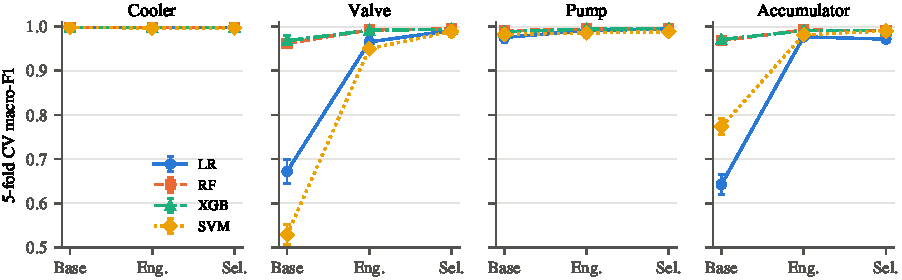
\includegraphics[width=\textwidth]{fig_cv_models.pdf}
\caption{Stratified 5-fold CV macro-F1 (training set) for each classifier and
input representation. Error bars show $\pm1$ standard deviation across folds.
Base: 17 channel means; Eng.: 553 descriptors; Sel.: 40 selected descriptors.}
\label{fig:cv}
\end{figure*}

\begin{table*}[t]
\centering
\caption{Stratified 5-fold CV macro-F1 on the training set (mean over folds). Bold: configuration selected for each target.}
\label{tab:cv}
\begin{tabular}{@{}llcccc@{}}
\toprule
Representation & Model & Cooler & Valve & Pump & Accumulator \\
\midrule
\multirow{4}{*}{Baseline ($d=17$)}
 & LR  & 0.9977 & 0.6722 & 0.9755 & 0.6424 \\
 & RF  & 0.9977 & 0.9621 & 0.9906 & 0.9684 \\
 & XGB & \textbf{0.9983} & 0.9682 & 0.9881 & 0.9706 \\
 & SVM & 0.9983 & 0.5287 & 0.9823 & 0.7735 \\
\midrule
\multirow{4}{*}{Full ($d=553$)}
 & LR  & 0.9977 & 0.9654 & 0.9911 & 0.9768 \\
 & RF  & 0.9977 & 0.9925 & 0.9943 & \textbf{0.9922} \\
 & XGB & 0.9977 & 0.9917 & 0.9946 & 0.9907 \\
 & SVM & 0.9966 & 0.9499 & 0.9855 & 0.9813 \\
\midrule
\multirow{4}{*}{Selected ($d=40$)}
 & LR  & 0.9983 & 0.9913 & 0.9947 & 0.9716 \\
 & RF  & 0.9977 & \textbf{0.9946} & 0.9954 & 0.9904 \\
 & XGB & 0.9983 & 0.9942 & \textbf{0.9954} & 0.9911 \\
 & SVM & 0.9972 & 0.9891 & 0.9886 & 0.9905 \\
\bottomrule
\end{tabular}
\end{table*}

\textit{Tree ensembles are robust to the representation.} On the 17 channel
means, RF and XGB already exceed 0.96 macro-F1 for every target, because
axis-aligned splits and learned interactions extract non-linear structure that
the means leave implicit.

\textit{Linear and kernel models depend strongly on it.} On the baseline, LR
scores 0.672 on the valve and 0.642 on the accumulator, and SVM 0.529 on the
valve. With the full representation, LR rises to 0.965 and 0.977; with the
selected 40 descriptors LR reaches 0.991 on the valve and SVM 0.989. The
information needed to separate these classes is present in the richer
representation in a form that is close to linearly separable.

\textit{Selection reduces dimension without cost.} Moving from 553 to 40
inputs changes the best score by at most 0.002 for any target and improves the
kernel and linear models on the valve and pump, which suffer most from
irrelevant dimensions. The cooler is solved by every model on every
representation (0.997--0.998), and the rule prefers the simplest option, a
17-input XGB model.

Fold-to-fold standard deviations of the selected configurations are
0.002--0.005, smaller than most between-model differences on the valve and
accumulator but comparable to the differences among the top three
configurations for every target. Rankings within 0.002 should therefore not be
over-interpreted.

\subsection{Held-Out Test Performance}
Table~\ref{tab:test} reports the single evaluation of each selected model on
its 441 test cycles. Cooler, valve and pump are classified without error. The
accumulator model reaches 0.989 accuracy and 0.988 macro-F1, with an ROC-AUC
of 0.9999, indicating that the remaining errors come from the decision
threshold rather than from poor ranking.

\begin{table}[t]
\centering
\caption{Selected models on the held-out test set (441 cycles each)}
\label{tab:test}
\begin{tabular}{@{}lllccc@{}}
\toprule
Target & Model & Input & Acc. & F1$_{\text{m}}$ & AUC \\
\midrule
Cooler & XGB & Base (17) & 1.000 & 1.000 & 1.000 \\
Valve & RF & Sel.\ (40) & 1.000 & 1.000 & 1.000 \\
Pump & XGB & Sel.\ (40) & 1.000 & 1.000 & 1.000 \\
Accumulator & RF & Full (553) & 0.989 & 0.988 & 0.9999 \\
\bottomrule
\end{tabular}
\end{table}

\subsection{Generalisation Gap Under Blocked Validation}
Fig.~\ref{fig:gap} and Table~\ref{tab:gap} compare random CV, blocked CV and
the test score. The ordering is consistent: blocked CV is lowest for every
target, and the gap grows with task difficulty, from 0.003 for the cooler to
0.076 for the accumulator. Since the test set was drawn by the same random
procedure as the CV folds, it shares their optimism, and the perfect test
scores are best read as an upper bound. Blocked CV is the more realistic
estimate of performance on cycles recorded at a different time, for example
after the rig has been run for a while.

\begin{figure}[t]
\centering
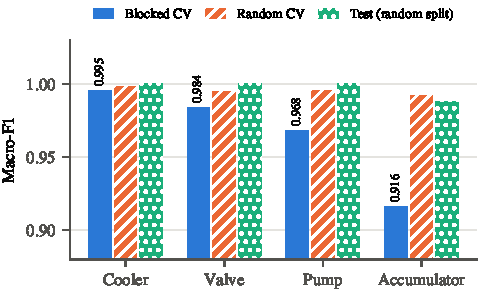
\includegraphics[width=\columnwidth]{fig_gap.pdf}
\caption{Macro-F1 of the selected model per target under blocked CV (blocks of
25 consecutive cycles), random stratified CV and the random-split test set.
The y-axis starts at 0.88.}
\label{fig:gap}
\end{figure}

\begin{table}[t]
\centering
\caption{Random vs.\ blocked 5-fold CV of the selected models}
\label{tab:gap}
\begin{tabular}{@{}lcccc@{}}
\toprule
 & \multicolumn{2}{c}{Macro-F1} & \multicolumn{2}{c}{Accuracy} \\
\cmidrule(lr){2-3}\cmidrule(lr){4-5}
Target & Random & Blocked & Random & Blocked \\
\midrule
Cooler & 0.998 & 0.995 & 0.998 & 0.995 \\
Valve & 0.995 & 0.984 & 0.996 & 0.987 \\
Pump & 0.995 & 0.968 & 0.997 & 0.979 \\
Accumulator & 0.992 & 0.916 & 0.993 & 0.933 \\
\bottomrule
\end{tabular}
\end{table}

\subsection{Error Analysis}
All five accumulator test errors are cycles with a true pre-charge of 100~bar
predicted as 90~bar (Fig.~\ref{fig:cm}); no other confusion occurs. The two
lowest pre-charge levels are adjacent on the physical scale, and a lower gas
pre-charge alters the pressure transients only slightly, so these two classes
are the most similar in feature space. This agrees with Helwig
\textit{et al.} \cite{helwig2015}, who also reported the lowest classification
rates for the accumulator. For maintenance the error is conservative: it overstates
degradation and would trigger an earlier inspection, not a missed failure.

\begin{figure}[t]
\centering
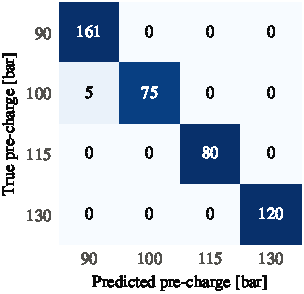
\includegraphics[width=0.72\columnwidth]{fig_cm_acc.pdf}
\caption{Test-set confusion matrix of the accumulator model (RF, 553 inputs).
Cell shading shows row-normalised recall.}
\label{fig:cm}
\end{figure}

\subsection{Interpretability}
Table~\ref{tab:imp} lists the inputs with the largest permutation importance
(mean drop in test macro-F1 over five random shuffles of one input column). The rankings are
physically plausible. The cooler model relies on the virtual cooling power CP
and on cooling efficiency, which directly express heat removal. The valve
model depends almost entirely on the coefficient of variation of pressure
PS2, consistent with switching lag distorting the pressure trace. The pump
model uses the upper quartile of flow FS1 and the peak motor power, since
internal leakage reduces delivered flow for the same electrical input.

The accumulator model is the exception: no single input has an importance
above 0.0011. With 553 highly correlated inputs, the forest spreads its splits
across many interchangeable descriptors, so shuffling any one of them is
compensated by the others. This is a known limitation of permutation
importance under collinearity and not evidence that the model uses no signal;
grouped importance or selection on this target would give a clearer picture.

\begin{table}[t]
\centering
\caption{Top inputs by permutation importance (test set)}
\label{tab:imp}
\begin{tabular}{@{}lll@{}}
\toprule
Target & Input & Importance \\
\midrule
Cooler & CP mean (cooling power) & 0.173 \\
       & PS2 mean & 0.008 \\
Valve  & PS2 coefficient of variation & 0.182 \\
       & PS2 std.\ of first difference & 0.007 \\
Pump   & FS1 75th percentile & 0.443 \\
       & EPS1 maximum & 0.093 \\
Accumulator & PS3 rolling-mean maximum & 0.001 \\
       & PS1 rolling-std maximum & 0.001 \\
\bottomrule
\end{tabular}
\end{table}

\subsection{Computational Cost}
Mean fit times per CV fold are below 0.9~s for all models on the 17-input
baseline, and between 0.06 and 9.1~s on the 553-input representation, where XGB
is the slowest (9.1~s on the accumulator). The selected pipelines take
1.4--3.1~s, most of it spent in the mutual-information and tree-importance
stages. Inference for one cycle, including descriptor extraction, runs in well
under a second, which is negligible relative to the 60-s cycle.

%=====================================================================
\section{Discussion and Limitations}
%=====================================================================
\textit{Selection on random CV.} Model selection used randomly split CV, while
blocked CV was computed only for the winner. A configuration that exploits
neighbouring-cycle similarity is favoured by this rule; the accumulator's
553-input forest, which has the largest optimism, may be one. Using blocked CV
as the selection criterion is the stricter design and is left to future work.

\textit{Single rig, laboratory faults.} All data come from one test rig with
deliberately set fault levels. Transfer to other machines, gradual in-service
degradation and simultaneous unseen faults is not established.

\textit{Virtual channels.} CE, CP and SE are computed by the rig's own model.
The cooler model's reliance on CP means its accuracy partly reflects that
model, and would need re-validation where such channels are unavailable.

\textit{Fixed hyperparameters.} Holding hyperparameters fixed makes the
comparison fair but may understate the linear and kernel models, whose
defaults are less forgiving than those of tree ensembles.

\textit{No remaining useful life.} The labels are condition levels without
run-to-failure information, so the system classifies current state and does
not forecast time to failure.

%=====================================================================
\section{Conclusion and Future Work}
%=====================================================================
Four classifier families were compared on four hydraulic condition targets
inside a leakage-safe pipeline. Tree ensembles are strong on every target and
representation, while linear and kernel models need the richer representation
to become competitive. The selected models classify cooler, valve and pump
without error on the held-out test set and reach 0.988 macro-F1 on the
accumulator, whose only confusion is between the two lowest pre-charge levels.
Blocked cross-validation lowers these estimates to 0.995, 0.984, 0.968 and
0.916, showing that randomly split scores on this dataset overstate
generalisation by up to 7.6 points and should be reported together with a
temporally aware estimate.

Future work will select models by blocked CV, add grouped feature
importance for the accumulator, explore a single multi-output model that
shares representation across targets, and test transfer to data recorded on
other hydraulic units.

%=====================================================================
\begin{thebibliography}{00}
\bibitem{helwig2015} N. Helwig, E. Pignanelli, and A. Sch\"{u}tze,
``Condition monitoring of a complex hydraulic system using multivariate
statistics,'' in \textit{Proc. IEEE Int. Instrum. Meas. Technol. Conf.
(I2MTC)}, Pisa, Italy, 2015, pp. 210--215,
doi: 10.1109/I2MTC.2015.7151267.

\bibitem{uci_hydraulic} N. Helwig, E. Pignanelli, and A. Sch\"{u}tze,
``Condition monitoring of hydraulic systems,'' UCI Machine Learning
Repository, 2015, doi: 10.24432/C5CW21.

\bibitem{carvalho2019} T. P. Carvalho, F. A. A. M. N. Soares, R. Vita,
R. P. Francisco, J. P. Basto, and S. G. S. Alcal\'{a}, ``A systematic
literature review of machine learning methods applied to predictive
maintenance,'' \textit{Comput. Ind. Eng.}, vol. 137, Art. no. 106024, 2019.

\bibitem{breiman2001} L. Breiman, ``Random forests,'' \textit{Mach. Learn.},
vol. 45, no. 1, pp. 5--32, 2001.

\bibitem{chen2016} T. Chen and C. Guestrin, ``XGBoost: A scalable tree
boosting system,'' in \textit{Proc. 22nd ACM SIGKDD Int. Conf. Knowl. Discov.
Data Min.}, 2016, pp. 785--794.

\bibitem{cortes1995} C. Cortes and V. Vapnik, ``Support-vector networks,''
\textit{Mach. Learn.}, vol. 20, no. 3, pp. 273--297, 1995.

\bibitem{pedregosa2011} F. Pedregosa \textit{et al.}, ``Scikit-learn: Machine
learning in Python,'' \textit{J. Mach. Learn. Res.}, vol. 12,
pp. 2825--2830, 2011.

\bibitem{kraskov2004} A. Kraskov, H. St\"{o}gbauer, and P. Grassberger,
``Estimating mutual information,'' \textit{Phys. Rev. E}, vol. 69, no. 6,
Art. no. 066138, 2004.

\bibitem{kaufman2012} S. Kaufman, S. Rosset, C. Perlich, and O. Stitelman,
``Leakage in data mining: Formulation, detection, and avoidance,''
\textit{ACM Trans. Knowl. Discov. Data}, vol. 6, no. 4, Art. no. 15, 2012.

\bibitem{roberts2017} D. R. Roberts \textit{et al.}, ``Cross-validation
strategies for data with temporal, spatial, hierarchical, or phylogenetic
structure,'' \textit{Ecography}, vol. 40, no. 8, pp. 913--929, 2017.
\end{thebibliography}

\end{document}
